\hypertarget{qlib_8h}{}\section{src/core/qlib.h File Reference}
\label{qlib_8h}\index{src/core/qlib.\+h@{src/core/qlib.\+h}}
{\ttfamily \#include \char`\"{}./general/object.\+hpp\char`\"{}}\\*
{\ttfamily \#include \char`\"{}./general/types.\+h\char`\"{}}\\*
{\ttfamily \#include \char`\"{}./math/complex.\+hpp\char`\"{}}\\*
{\ttfamily \#include \char`\"{}./math/matrix.\+hpp\char`\"{}}\\*
{\ttfamily \#include \char`\"{}./quantum/systems/qubit.\+hpp\char`\"{}}\\*
{\ttfamily \#include \char`\"{}./quantum/systems/qreg.\+hpp\char`\"{}}\\*
{\ttfamily \#include \char`\"{}./quantum/standard\+\_\+gates.\+hpp\char`\"{}}\\*
{\ttfamily \#include \char`\"{}./quantum/systems/system.\+hpp\char`\"{}}\\*
{\ttfamily \#include \char`\"{}./quantum/systems/ensemble.\+hpp\char`\"{}}\\*
Include dependency graph for qlib.\+h\+:\nopagebreak
\begin{figure}[H]
\begin{center}
\leavevmode
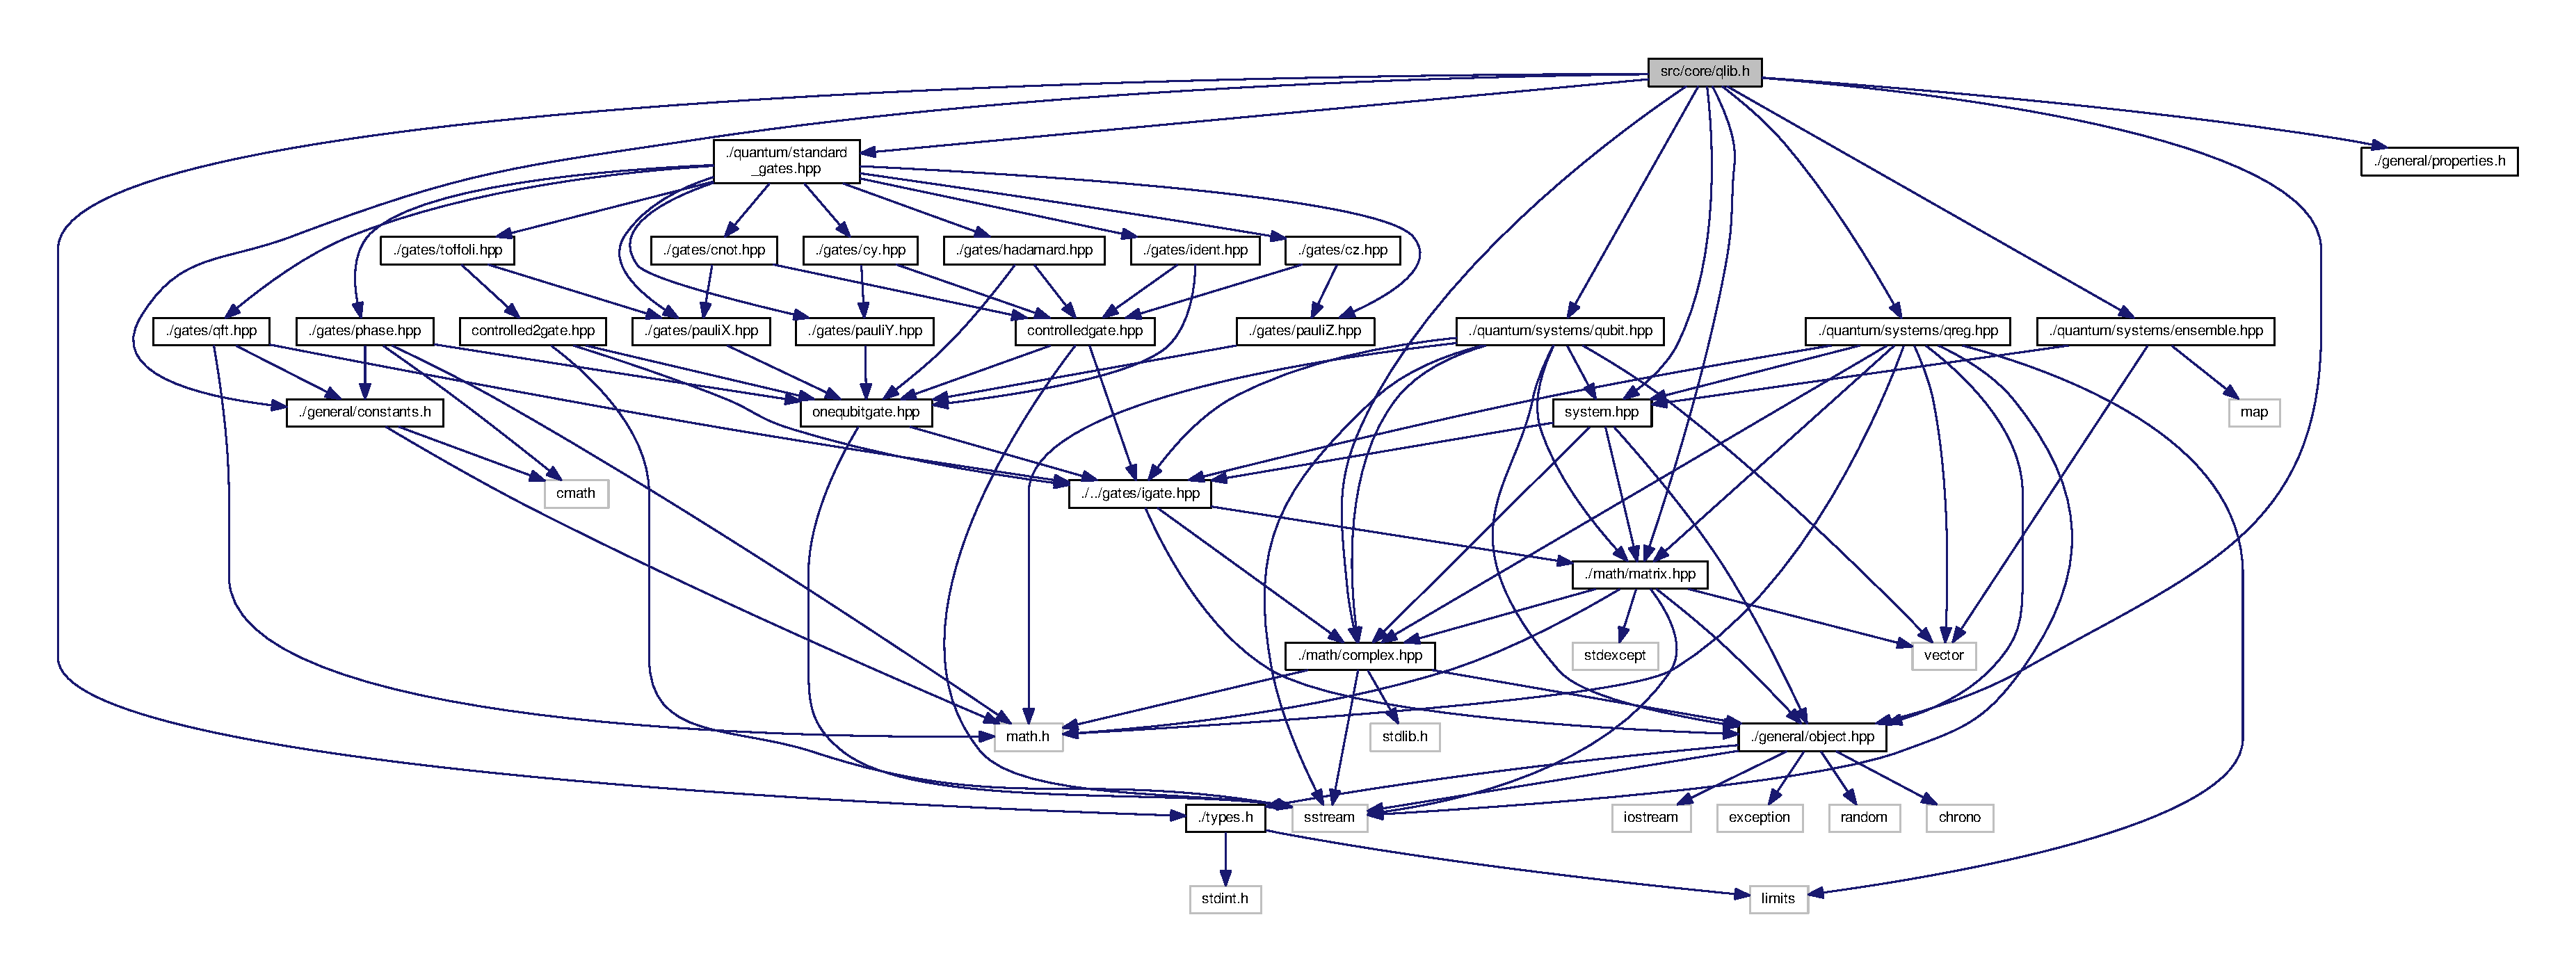
\includegraphics[width=350pt]{qlib_8h__incl}
\end{center}
\end{figure}
This graph shows which files directly or indirectly include this file\+:\nopagebreak
\begin{figure}[H]
\begin{center}
\leavevmode
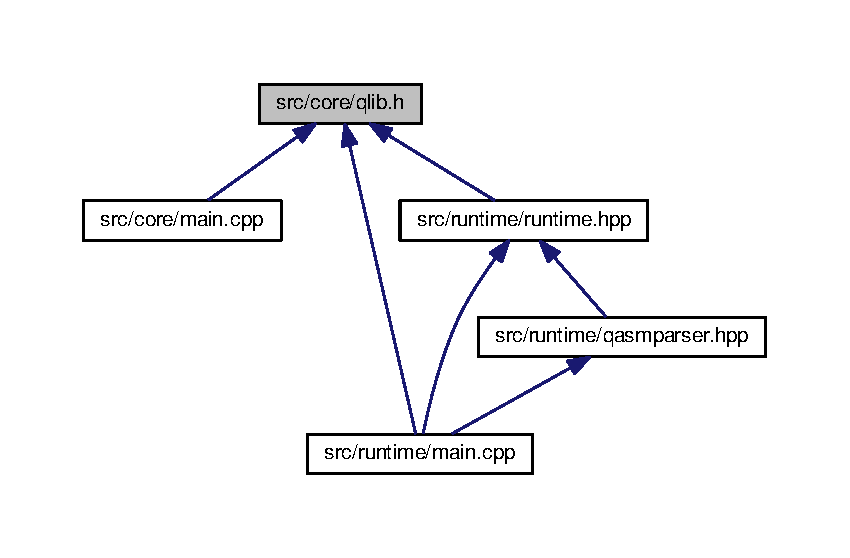
\includegraphics[width=350pt]{qlib_8h__dep__incl}
\end{center}
\end{figure}
